\documentclass[../main.tex]{subfiles}

\begin{document}

\section{Exploding brains in Julia}

\authors{\"Omer Faruk G\"ulban\textsuperscript{1,2}, Leonardo Muller-Rodriguez\textsuperscript{3}}

\affiliations{1. Department of Cognitive Neuroscience, Faculty of Psychology and Neuroscience, Maastricht University, Maastricht, The Netherlands, 2. Brain Innovation, Maastricht, The Netherlands, 3. Psychoinformatics Lab, Forschungszentrum J\"ulich, J\"ulich, Germany}

Particle simulations are used to generate visual effects (in movies, games etc...). In this project, we explore how we can use magnetic resonance imaging (MRI) data to generate interesting visual effects by using (2D) particle simulations. We highlight that, historically, we were first inspired by a detailed blog post (\texttt{\url{https://nialltl.neocities.org/articles/mpm_guide.html}}) on the material point method \parencite{Jiang1965, Love2006, Stomakhin2013a}. Our aim in Brainhack 2022 is to convert our previous progress in Python programming language to Julia. The reason why we have moved to Julia language is because it has convenient parallelization methods that are easy to implement while giving immediately speeding-up the particle simulations.

-----------------------------------

Our previous efforts are documented at:
\begin{enumerate}
    \item 2020 OpenMR Benelux: \texttt{\url{https://github.com/OpenMRBenelux/openmrb2020-hackathon/issues/7}} 
    \item 2020 OHBM Brainhack: \texttt{\url{https://github.com/ohbm/hackathon2020/issues/124}}
    \item Available within the following github repository: \texttt{\url{https://github.com/ofgulban/slowest-particle-simulator-on-earth}}    
\end{enumerate}

-----------------------------------

As a result of this hackathon project, a compilation of our progress (\Cref{fig:exploding_brains}) can be seen at \texttt{\url{https://youtu.be/_5ZDctWv5X4}} as a video. Our future efforts will involve sophisticating the particle simulations, the initial simulation parameters to generate further variations of the visual effects, and potentially synchronizing the simulation effects with musical beats.

\begin{figure}
	\centering
	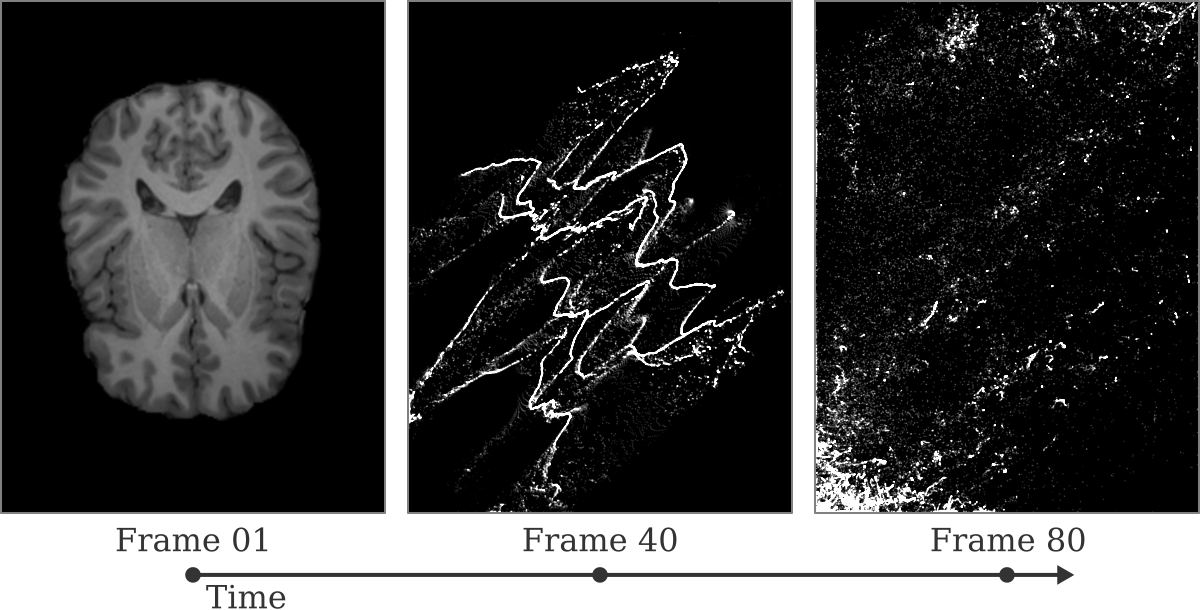
\includegraphics[width=0.5\textwidth]{images/exploding_brains.png}
	\caption{A video compilation of brain explosions can be seen at \texttt{\url{https://youtu.be/_5ZDctWv5X4}}.}
	% Add a label to reference in text. Make it specific!
	\label{fig:exploding_brains}
\end{figure}

\printbibliography


\end{document}
